%%%%%%%%%%%%%%%%%%%%%%%%%%%%%%%%%%%%%%%%% 
\documentclass{eajam}
%%%%% journal  info %%%%%%%%%
\setcounter{page}{1}
\renewcommand\thisnumber{x}
\renewcommand\thisyear {2016}
\renewcommand\thismonth{xxx}
\renewcommand\thisvolume{xx}
%%%%%%%%   end  %%%%%%%%%%%%%

%%%%% author macros %%%%%%%%%
% place your own macros HERE
%%%%% end %%%%%%%%%

\usepackage{graphicx} % Required for the inclusion of images
\usepackage{epstopdf} % eps to pdf
\usepackage{epsfig}
\usepackage{amsmath} % Required for some math elements 
\usepackage[colorlinks, linkcolor=black, anchorcolor=blue,
citecolor=black]{hyperref}
\usepackage{algorithm}
\usepackage{algpseudocode}
\usepackage{tikz}
\usepackage{pgflibraryarrows}
\usepackage{pgflibrarysnakes}
\usepackage{subfig}
\usepackage{booktabs}
% table 环境中的多行.
\usepackage{multirow}
% ----------------------------------------------------------------------------------------
%	DOCUMENT INFORMATION
% ----------------------------------------------------------------------------------------
\begin{document}

%%%%% title and author(s):
% \markboth{Author(s)}{Short Title}
% \title{Title}

\markboth{Yirong Wu and Heyu Wang}{Moving mesh FEM for unsteady NS flow}
\title{AMG preconditioner for moving mesh finite element method}

% single author:
% \author[AUTHOR]{AUTHOR\corrauth}
% \address{address of AUTHOR}
% \email{{\tt email address of AUTHOR} (AUTHOR)}
%\author[Only Author]{Only Author\corrauth}
%\address{School of Mathematical Sciences, Beijing International University,
%Beijing 12345, China.}
%\email{{\tt email@address} (Only Author)}

% multiple authors:
% Please mark \corrauth after the name of the corresponding author.
% different addresses:
%\author[AUTHOR1 and AUTHOR2]{AUTHOR1\affil{1}\comma\corrauth and AUTHOR2\affil{2}}
%\address{\affilnum{1}\ address of AUTHOR1\\
%\affilnum{2}\ address of AUTHOR2}
%
%same address:
%\author[AUTHOR1, AUTHOR2 and AUTHOR3]{AUTHOR1, AUTHOR2\corrauth and AUTHOR3}
%\address{address of AUTHOR1, AUTHOR2 and AUTHOR3}
%
%\emails{{\tt email of AUTHOR1} (AUTHOR1), {\tt email of AUTHOR2} (AUTHOR2), {\tt email of AUTHOR3} (AUTHOR3)}
%
%same address:
\author[Yirong Wu and Heyu Wang]{Yirong Wu and Heyu Wang\corrauth}
\address{School of Mathematical Science, ZheJiang University, HangZhou,
  310027, China}

\emails{{\tt wuwuyiyirongrong@163.com} (Yirong Wu), {\tt
    wang.heyu@gmail.com} (Heyu Wang)}

%%%%% Begin Abstract %%%%%%%%%%%
\begin{abstract}
    In this paper, we apply an AMG prconditioner to solve
    the unsteady Navier-Stokes equations with moving mesh finite
    element method. $4P1-P1$ element pair is selected, which based on
    the data structure of hierarchy geometry tree. We choose two-layer nested
    meshes that velocity mesh and pressure mesh. An AMG preconditioner
    is designed for PDE solver and divergence-interpolation in moving
    mesh strategy. Numerical experiments shown the efficiency of the
    AMG preconditoner for moving mesh finite element. \\
\end{abstract}
%%%%% end %%%%%%%%%%%

%%%%% Keywords %%%%%%%%%%%
\keywords{Navier-Stokes, algbraic multigrid precondition, moving mesh.}

%%%% maketitle %%%%%
\maketitle

%%%% Start %%%%%%
\section{Introduction}
    \label{sec1} The incompressible Navier-Stokes equations in
    primitive variables are 
    \begin{equation}
      \begin{array}{rcl}
         \partial_t \vec{u} - \nu \nabla^2 \vec{u} +
        (\vec{u} \cdot \nabla )\vec{u} + \nabla p & =
        & \vec{f},\\
        \nabla \cdot \vec{u} & = & 0,
      \end{array}
      \label{eq::NS}
    \end{equation}
    with initial and boundary conditions on $\partial
    \Omega = \partial \Omega_D \bigcup \partial \Omega_N$:
    \begin{equation}
      \begin{array}{ll}
        \vec{u} = \vec{w},& \mbox{ on } \partial \Omega_D \times [0,
        T]\\
        \nu \displaystyle \frac{\partial \vec{u}}{\partial n} - p =
        \vec{0}, & \mbox{ on } \partial \Omega_N \times [0, T],  \\
        \vec{u}|_{t = 0} = \vec{u_0}, & \mbox{ in } \Omega. 
      \end{array}
      \label{eq::bc}
    \end{equation}    
    where $\Omega \in \mathcal{R}^d,(d = 2, 3)$ is computional domain,
    $[0,T]$ is the time interval, $\vec{u}$ is velocity and scalar $p$
    is pressure, $\vec{n}$ denotes outward normal direction of
    $\partial \Omega$, $\nu > 0$ is the constant kinematic
    viscosity.

    We solve equations (\ref{eq::NS}) and (\ref{eq::bc}) by moving
    mesh finite element methods based on \cite{li2001mesh} and
    \cite{di2005}. In the past, some moving methods have been
    introduced. Winslow \cite{Winslow1966NUMERICAL} proposed solving
    elliptic PDEs using moving mesh. As an extension of Winslow' work,
    Dvinsky \cite{dvinsky1991adaptive} pointed out that harmonic
    function theory could be used for generating mesh. Motivated by
    Dvinsky's work, L1, Tang and Zhang \cite{li2001mesh} proposed a
    moving mesh finite element strategy based upon harmonic
    mapping. The authors in \cite{di2005moving} extended the moving
    strategy to solve the incompressible Navier-Stokes equations in
    primitive variables. The author designed a divergence-free
    interpolation in moving strategy by solving a linearized
    Navier-Stokes-type equations. In \cite{Wu2016moving}, $4P1-P1$
    element pair is applied to solve incompressible Navier-Stokes flow
    with moving mesh finite element method based on the work of
    \cite{di2005moving}. This pair has same mesh structure as
    $P1isoP2P1$ element, which is natrually LBB stable see
    \cite{bercovier1979error}. Four velocity elements can be obtained
    by refining the pressure element one time see Figure
    \ref{fig::p-v}. Linear velocity basis functions of
    $4P1-P1$ are all locally in the same velocity element, whereas
    $P1isoP2P1$ not, see \cite{Wu2016moving} for detail.

    As we known, spacial discretization of Navier-Stokes system with
    LBB-stable $4P1-P1$ element pair leads to a saddle point problem.
    There are a lot works on saddle point problems by developing
    preconditioners for Krylov subspace method, such as block
    preconditioner and multigrid strategy. Readers can refer to
    \cite{benzi2005numerical} for detail. Many works(
    \cite{bai2005inexact}, \cite{bai2006structured},
    \cite{elman2007least},\cite{elman2009boundary}) introduce a
    variety of block preconditioners, whose main issue are finding a
    good approximation of schur complement. Also there are other
    precondition methods, for instance (\cite{benzi2006augmented},
    \cite{benzi2011relaxed}). The authors in (\cite{boyle2007hsl}
    \cite{boyle2010hsl_mi20}) propose an efficient AMG preconditioner
    for Krylov solver to solve Navier-Stokes equations. However,
    efficient precondition methods for saddle point problems are nearlly
    based on uniform mesh (although \cite{benzi2011relaxed} considered
    the stretched mesh case).
    
    In this work, we apply an AMG preconditioner to moving mesh
    finite element for solving systems (\ref{eq::NS}) and
    (\ref{eq::bc}) based on the work of
    \cite{elman2005finite}. Efficiency of the AMG preconditioner is 
    analyzed througth several numerical experiments.

    \begin{figure}
      \centering    
      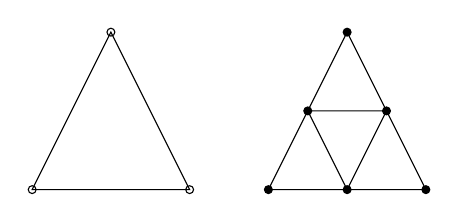
\begin{tikzpicture}
        % 三角形
        \draw (2, 1) -- (4, 1) -- (3, 3) -- cycle;
        % 三个顶点
        \draw (2, 1) circle(0.05cm);
        \draw (4, 1) circle(0.05cm);
        \draw (3, 3) circle(0.05cm);
        % 四个三角形
        \draw (5, 1) -- (6, 3) -- (7, 1) -- cycle;
        \draw (5.5, 2) -- (6.5, 2) -- (6, 1) -- cycle;
        % 六个顶点
        \draw [fill = black] (5, 1) circle(0.05cm);
        \draw [fill = black] (6, 3) circle(0.05cm);
        \draw [fill = black] (7, 1) circle(0.05cm);
        \draw [fill = black] (5.5, 2) circle(0.05cm);
        \draw [fill = black] (6.5, 2) circle(0.05cm);
        \draw [fill = black] (6, 1) circle(0.05cm);
      \end{tikzpicture}
      \caption{Left: pressure $p$ element, $\circ$ for degrees of $p$; 
               right: four velocity $v$ elements, $\bullet$ for degrees
               of $v$.}
      \label{fig::p-v}       
    \end{figure}
      
       The layout of the paper is arraged as follows. In
    section 2, we use $4P1-P1$ elements to approximate the governing
    equations. Next, the AMG preconditioner for
    Navier-Stokes equations is shown. In Section 4, we give the moving mesh
    strategy briefly. Then we present numerical experiements in section 5. 
    Finaly, we give the conclusions in this section.

% ----------------------------------------------------------------------------------------
%	SECTION 1
% ----------------------------------------------------------------------------------------
\section{Finite Element Discretization}
   \label{sec2} At time level discretization, we devide the time
   interval $[0, T]$ into $N$ steps with $\{ t_i\}_{i = 1}^N$. Let
   $\vec{u}^j$ and $p^j$ be the discrete approximation to
   $\vec{u}(\cdot, t_j)$ and $p(\cdot, t_j)$. For simplicity, we
   choose linear backward Euler scheme that linearizing the
   nonlinear term $(\vec{u}^{n + 1} \cdot \nabla) \vec{u}^{n + 1}$
   with $(\vec{u}^n \cdot \nabla) \vec{u}^{n + 1}$.

   In this work, we adopt finite element pair $4P1-P1$,
   which based on two different trianglar meshes and two different
   finite element spaces. By using the hierarchy geometry tree
   (\cite{li2005multi}) structure, velocity mesh can be
   obtained via global refining pressure mesh one time see Figure
   \ref{fig::hgeometry_tree}.
   
   \begin{figure}[h]
     \subfloat[One time uniform refined mesh]{
       \begin{minipage}[t]{0.4\textwidth}
         \centering
         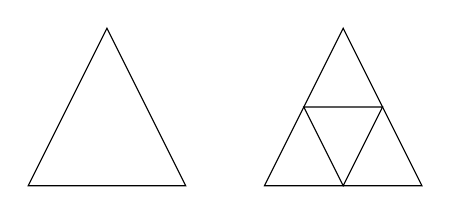
\begin{tikzpicture}
           % 三角形
           \draw (2, 1) -- (4, 1) -- (3, 3) -- cycle;
           \draw (5, 1) -- (6, 3) -- (7, 1) -- cycle;
           \draw (5.5, 2) -- (6.5, 2) -- (6, 1) -- cycle;
         \end{tikzpicture}
       \end{minipage}
     }
     \subfloat[its hierarchy tree]{
       \begin{minipage}[t]{0.6\textwidth}
         \centering
         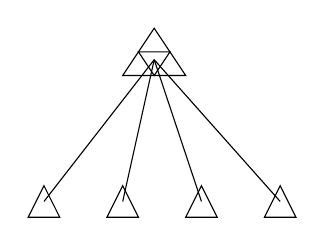
\begin{tikzpicture}
           %五个小三角形
           \draw (1.0, 0.0) -- (1.2, 0.4) -- (1.4, 0.0) -- cycle;
           \draw (2.0, 0.0) -- (2.2, 0.4) -- (2.4, 0.0) -- cycle;
           \draw (3.0, 0.0) -- (3.2, 0.4) -- (3.4, 0.0) -- cycle;
           \draw (4.0, 0.0) -- (4.2, 0.4) -- (4.4, 0.0) -- cycle;
           \draw (2.6, 2.4) -- (2.2, 1.8) -- (3.0, 1.8) -- cycle;
           \draw (2.4, 2.1) -- (2.6, 1.8) -- (2.8, 2.1) -- cycle;
           %四条线
           \draw (2.6, 2.0) -- (1.2, 0.2);
           \draw (2.6, 2.0) -- (2.2, 0.2);
           \draw (2.6, 2.0) -- (3.2, 0.2);
           \draw (2.6, 2.0) -- (4.2, 0.2);
         \end{tikzpicture}
       \end{minipage}
     }
     \caption{Hierachy tree structure}
     \label{fig::hgeometry_tree}
   \end{figure}

   The $1-1$ index between velocity elements and pressure elements can
   be obtained without difficulties with the hierarchy geometry tree
   structure. Interested author see \cite{Wu2016moving} for
   details. First some notification are denoted as
   fowllows. $\mathcal{T}_h$ is the grid triangulation
   division for velocity mesh with mesh size $h = max_{T \in
     \mathcal{T}_h} diam(T)$, while $\mathcal{T}_{H}(H = 2h)$ for
   pressure mesh. $\mathcal{X}_h \subset (\mathcal{H}_0^1(\Omega)^2)$ and
   $P_H \subset \mathcal{L}^2(\Omega)$ are finite-dimentional
   approximation spaces. Then the full discretization is the
   following: given$(\vec{u}_h^n, p_H^n)$ at time $t_n$, to compute
   $(\vec{u}_h^{n + 1}, p_H^{n + 1})$ via 
   \begin{equation}
     \begin{aligned}
       \frac{1}{dt}(\vec{u}_h^{n + 1}, \vec{v}_h) + \nu (\nabla
       \vec{u}_h^{n + 1}, \nabla \vec{v}_h) + (\vec{u}_h^n \cdot
       \nabla \vec{u}_h^{n + 1}, \vec{v}_h) - (p_H^{n + 1}, \nabla
       \vec{v}_h) & = &\frac{1}{dt}(\vec{u}_h^n, \vec{v}) \\
       (\nabla \cdot \vec{u}_h^{n + 1}, q_H) & = & 0. \\
     \end{aligned}
     \label{eq::NS_weak_form}
   \end{equation}
   
   for all $(\vec{v}_h, q_H) \in \mathcal{X}_h \times P_H$.

\section{Fast Krylov Solver}
  \label{sec3} Let $\left(\{\phi_j \}_{j = 1}^n, 0 \right)^T$ and
  $\left(0, \{\phi_j\}_{j = 1}^n\right)^T$ be linear basis functions
  for velocity space $\mathcal{X}_h$. Meanwhile, $\{\psi_k\}_{k =
    1}^m$ denotes linear basis functions for pressure space
  $\mathcal{M}_H$. Then components of velocity solutions
  $\vec{u}_h^{n + 1} = (u_h^{x, n + 1}, u_h^{y, n + 1})^T$ and pressure
  solution $\vec{p}_H^{n + 1}$ at $t = t_{n + 1}$ can be written as 
  \begin{equation}
    u_h^{x, n + 1} = \sum_{j = 1}^{n_u} \alpha_j^{x, n + 1} \phi_j,
    \qquad u_h^{y, n + 1} = \sum_{j = 1}^{n_u} \alpha_j^{y, n + 1}
    \phi_j \qquad p_H^{n + 1} = \sum_{k = 1}^{n_p}\alpha_k^{p, n + 1}
    \psi_k.
    \label{eq::basis_fun}
  \end{equation}
  
  substituting (\ref{eq::basis_fun}) inito weak form
  (\ref{eq::NS_weak_form}), saddle-point system can be obtained
  
  \begin{equation}
    \left[
      \begin{array}{lll}
        \frac{1}{dt} M + \nu A + N & 0 & B_x^T \\
        0 & \frac{1}{dt} M +\nu A + N  & B_y^T \\
        B_x & B_y & 0
      \end{array}
    \right]
    \left[
      \begin{array}{c}
        \alpha^{x, n + 1} \\
        \alpha^{y, n + 1} \\
        \alpha^{p, n + 1}
      \end{array}
    \right] = 
    \left[
      \begin{array}{c}
        f_x \\
        f_y \\
        0
      \end{array}
    \right],
    \label{eq::linear_system}
  \end{equation} 
  Notice that divergence matrix $B = [Bx, By]$ is 
  \begin{eqnarray}
    B_x := [B_x]_{kj} = -\left(\psi_k, \frac{\partial \phi_j}{\partial
        x} \right), k = 1, \cdots, n_p, j = 1, \cdots, n_u, \\
    B_y := [B_y]_{kj} = -\left(\psi_k, \frac{\partial \phi_j}{\partial
        y} \right), k = 1, \cdots, n_p, j = 1, \cdots, n_u.
  \end{eqnarray}
  Assembling of matrix $B$ is a non-trival process due to the
  basis functions of velocity elements and pressure elements are on 
  different mesh. According to the $1-1$ index between velocity
  elements and pressure elements metioned above, we can just use local
  $P1$ element of both velocity and pressure elements to assemble $B$.
  $B^T$ is in the same way.
  
  We denote $F_\nu^{n + 1} = \frac{1}{dt} M + \nu A + N$, where
  \begin{eqnarray}
    M := &[M]_{ij} =& \left( \phi_i, \phi_j \right),\quad  i,j = 1, \cdots,
    n_u, \\
    A := &[A]_{ij} =& \left( \nabla \phi_i, \nabla \phi_j \right), i,j =
    1, \cdots, n_u, \\
    N := &[N]_{ij} =& \left(\vec{u}_h^n, \nabla \phi_i, \phi_j \right),
    i,j = 1, \cdots, n_u.
  \end{eqnarray}
  
  To solve linear system \ref{eq::linear_system} efficiently, we 
  use preconditioned GMRES as solver. The block trianglar
  preconditioner $\mathcal{P}$ discussed in \cite{elman2005finite}
  which is defined as following
  \begin{equation}
    \mathcal{P} = 
    \left( 
      \begin{array}{lll}
        F & 0 & B_x^T \\
        0 & F  & B_y^T \\
        0 & 0 & S
      \end{array}
    \right)
  \end{equation}
  where $S = B_xF^{-1}B_x^T + B_yF^{-1}B_y^T$ is the schur complement
  matrix. The action of $\mathcal{P}^{-1}$ is divided into two steps:
  first, solve schur complement system, second, solve two scalar
  system associated with $F$. It is costly to directly solve schur
  complement system. So in practical computation, the PCD
  preconditioner discussed in \cite{elman2005finite} is used to
  approximate schur complement matrix $S$. PCD preconditioner is
  denoted as $S_* = A_p F_p^{-1} Q_p$ where $A_p, F_p$ and $Q_p$ are
  all on the pressure space. $Q_p$ is mass matrix, $A_p$ is pressure
  diffusion matrix and $F_p$ is convection diffusion matrix denoted as
  \begin{eqnarray}
    F_p := [F_p]_{ij} = \nu (\nabla \psi_i, \nabla \psi_j) +
    (\vec{u}_h^n \cdot \nabla \psi_i, \psi_j), \quad i,j = 1, \cdots, n_p, \\
    A_p := [A_p]_{ij} = (\nabla \psi_i, \nabla \psi_j)\quad i,j = 1, \cdots,
    n_p.
    \label{eq::pcd_mat}
  \end{eqnarray}
  Let $W_p^n := [W_p^n]_{ij} = (\vec{u}_h^n \cdot \nabla \psi_i,
  \psi_j), \quad i,j = 1, \cdots, n_p$, then $F_p$ can be rewitten as
  $F_p = \nu A_p + W_p^n$. We implement PCD preconditioning by 
  \begin{equation}
    S_*^{-1} \approx Q_p^{-1} F_p A_p^{-1}.
  \end{equation}
  Exact PCD preconditioning opearator is denoted as 
  \begin{equation}
    \mathcal{M}^{-1} = 
    \left(
      \begin{array}{lll}
        F^{-1} & 0 & B_x^T \\
        0 & F^{-1} & B_y^T \\
        0 & 0 &S_*^{-1}
      \end{array}
    \right)
  \end{equation}
  In practical computation, we use a fixed number of AMG iterations
  for matrix $F$, $F_p$, $Q_p$, and $A_p$ to replace exact solving,
  which refers to iterated PCD preconditioning. The AMG solver is
  based on the AFPack(a adaptive finite element pack) which can be
  obtained from \url{http://dsec.pku.edu.cn/~rli}. The efficiency of
  PCD preconditioning is shown in (\cite{elman2005finite},
  Section 10) and (\cite{elman2011fast}) for bouyancy driven flow
  problem. In our experiements, $F_p$ in (\ref{eq::pcd_mat}) is not so
  efficient as getting rid of $\nu$ in (\ref{eq::pcd_mat}). If without
  explanation, we refer $F_p = A_p + W_p^n$ in this paper. We compare
  the efficiency of two choice of $F_p$ in numerical test below. We
  adopt the method in \cite{elman2009boundary} to deal with matrixes
  $F_p$ and $A_p$ on Neumann boundary for improving efficiency.
  
  In this work, we apply the PCD preconditioning strategy to moving mesh
  finite element method to efficiently solve system
  (\ref{eq::linear_system}). The moving strategy will be shown in next
  section.
 
\section{Moving Mesh Strategy}
   \label{sec4} We refer the moving strategy to
   \cite{di2005moving}. In the following, we briefly introduce the
   moving mesh method. At time $t = t_{n}$, we obtain  numerical
   solutions $\vec{u}_h^{(n)}, p_H^{(n)}$ on old 
   mesh $\mathcal{T}_h^n$. We follow the framework in
   \cite{di2005moving} to implement divergence-free 
   interpolation of solutions on $\mathcal{T}_h^n$ to new mesh
   $\mathcal{T}_h^{(n + 1)}$. Briefly speaking, the moving mesh
   strategy mainly contains four steps as follows.
   \subsection{Step 1 Obtain monitor function}
      It is very important to choose an appropriate monitor function for
      adaptive scheme. Let $m = 1/G$, where $G$ is the monitor
      function. As illustrated in \cite{di2005moving}, there are some
      common choices of $G$. One based on vorticity is 
      \begin{equation} 
        \centering
        G_0 = \sqrt{1 + \alpha |\omega|^\beta}.
        \label{eq::monitor_vorticity}
      \end{equation}
      where $\omega = \nabla \times \vec{u}$, $\alpha, \beta$
      are positive constants. In this work, $\beta = 2$ performs 
      well, while $\alpha$ is user defined according to different
      problems. 
   \subsection{Step 2 Get a new logical mesh}
      Solve elliptic equation 
      \begin{eqnarray}
        \nabla_{\vec{x}}(m \nabla_{\vec{x}} \vec{\xi}) = 0, \\
        \vec{\xi}|_{\partial \Omega} = \vec{\xi}_b.
        \label{eq::logical}
      \end{eqnarray}
      where $m$ is given in step 1. Then a new logical mesh
      $\mathcal{T}_c^*$ with $\mathcal{A}^*$ as nodes is obtained.

   \subsection{Step 3 Achieve mesh move direction in physical domain}
      First, some notaions are introduced. $\mathcal{T}_h$ is the
      triangulation of physical domain, $X_i$ is the $i$-th node and  
      $T_i$ denotes the set of elements containing $X_i$.
      The notations on the logical domain are seperatly
      $\mathcal{T}_c, \mathcal{A}_i, T_{i, c}$. $(\mathcal{A}_i^1,
      \mathcal{A}_i^2)$ are the coordinates of $\mathcal{A}_i$ the
      $i$-th node in the logical domain. After Step 1 and
      Step 2, we obtain a new logical mesh $\mathcal{T}_c^*$,
      meanwhile $\mathcal{A}_i^*$ as its $i$-th node. Then we can get
      the error on the $i$-th node:
      \begin{equation}
        \delta \mathcal{A}_i = \mathcal{A}_i^0 - \mathcal{A}_i^*
      \end{equation}
      in which  $\mathcal{A}_i^0$ denotes the $i$-th node of the
      initial logical mesh $\mathcal{T}_c^0$. Noticing that once the
      initial logical mesh obtained, it doesn't change until the whole
      algorithm is over.
      
      For a given element $E$ in $\mathcal{T}_h$,  $X_k, 0 \leq k \leq
      2$ denotes it's vertexes. We can get the piecewise linear map from
      $V_{T_c^*}(\Omega_c)$ to $V_T(\Omega)$, which has constant gradient 
      $\partial \vec{x} / \partial \xi $ on E, via solving following
      system
      \begin{eqnarray}
        \begin{aligned}
          & \left (
            \begin{array}{cc}
              \mathcal{A}_{E_1}^{*, 1} - \mathcal{A}_{E_0}^{*, 1} & 
              \mathcal{A}_{E_2}^{*, 1} - \mathcal{A}_{E_0}^{*, 1} \\
              \mathcal{A}_{E_1}^{*, 2} - \mathcal{A}_{E_0}^{*, 2} &
              \mathcal{A}_{E_2}^{*, 2} - \mathcal{A}_{E_0}^{*, 2} 
            \end{array} 
          \right )
          \left (
            \begin{array}{cc}
              \frac{\partial x^1}{\partial \xi^1} & \frac{\partial
                x^1}{\partial \xi^2} \\
              \frac{\partial x^2}{\partial
                \xi^1} & \frac{\partial x^2}{\partial \xi^2}
            \end{array}
          \right ) \notag \\ = & 
          \left (
            \begin{array}{ll}
              X_{E_1}^1 - X_{E_0}^1 & X_{E_2}^1 - X_{E_0}^1 \\
              X_{E_1}^2 - X_{E_0}^2 & X_{E_2}^2 - X_{E_0}^2 
            \end{array}
          \right )
        \end{aligned}
      \end{eqnarray}
      The weighted average displacement of the $i$th node $X_i$ is as
      follows:
      \begin{eqnarray}
        \delta X_i = \frac{\sum\limits_{E \in T_i} |E| \frac{\partial
            \vec{x}}{\partial \xi}|_{\text{in} E} \delta
          \mathcal{A}_i}{\sum\limits_{E \in T_i} |E|}.
      \end{eqnarray}
      where the weight $|E|$ denotes the volume of element $E$.
      Meanwhile a positive parameter $\mu$ is multiplied to the 
      displacement $\delta X_i$ to prevent mesh
      tangling. Let $\mathcal{T}^*$ be the new mesh on the physical
      domain with nodes $X_i^*$
      \begin{equation}
        X_i^* = X_i + \mu \delta X_i
      \end{equation}
      The selecting $\mu$ is detailedly introduced in \cite{di2005moving}. 
   \subsection{Step 4 Eusure the incompressible constraint interpolation}
      It is necessary to keep divergence-free in the interpolation
      when solving incompressible flow with moving mesh finite element
      method. In \cite{di2005moving}, solution re-distribution on the new 
      mesh $\mathcal{T}^*$ is achieved via solving a lineard inviscid 
      Navier-Stokes-type equations as following
      \begin{eqnarray}
        \begin{aligned}
          \frac{\partial \vec{u}}{\partial \tau} - \nabla_{\vec{x}}\vec{u}
          \cdot \delta \vec{x} & = & - \nabla \hat{p}. \\
          \nabla_{\vec{x}}\cdot \vec{u} & = & 0
        \end{aligned}
        \label{eq::continous_update}
      \end{eqnarray} 
      where $\delta \vec{x} := x^{\text{old}} - x^{\text{new}}$ and 
      $x^{\text{old}}, x^{\text{new}}$ are two sets of coordinates in
      physical domain. $\tau$ is a virtual time variable and often
      choosen as $1.0$, because of the convection speed $\delta \vec{x}$
      is relatively small. Here $\hat{p}$ is a temporary variable
      distinguished from pressure variable in (\ref{eq::NS}). 

      Weak form of (\ref{eq::continous_update}) is : find $(\vec{u}_h,
      \hat{p}_H) \in X_E^h \times P^H$ such that 
      \begin{eqnarray}
        \begin{aligned}
          \left( \partial_{\tau} \vec{u}_h - \nabla_{\vec{x}}\vec{u}_h
            \cdot \delta \vec{x}, \vec{v}_h \right) & = & \left( \hat{p}_H, \nabla
            \vec{v}_h \right), \quad \forall \vec{v}_h \in X_E^h. \\
          \left( \nabla_{\vec{x}} \cdot \vec{u}, q_H\right) & = & 0, \quad \forall
          q_H \in P^H.
        \end{aligned}
        \label{eq::semi_discreted_update}
      \end{eqnarray}
      
      In this work, we use explicit scheme to
      (\ref{eq::semi_discreted_update}) for time discretization:
      \begin{eqnarray}
        \begin{aligned}
          \left ( \frac{\vec{u}_{h, *}^{(n)} - \vec{u}_h^{(n)}}{\delta
            t},
            \vec{v}_h \right) + \left( \delta \vec{x} \cdot \nabla 
            \vec{u}_{h}^{(n)}, \vec{v}_h \right)  & = & \left( 
            \hat{p}_{H, *}^{(n)}, \nabla \vec{v}_h \right), \quad
          \forall \vec{v}_h \in X_E^h. \\
          \left( \nabla \cdot \vec{u}_{h, *}^{n}, q_H \right) & = & 0, \quad
          \forall q_H \in P^H.
        \end{aligned}
        \label{eq::full_discreted_update}
      \end{eqnarray}
      where $\vec{u}_h^{(n)}$ and $p_H^{(n)}$ are the numerical
      solutions of (\ref{eq::NS}) at $t = t_{n}$ using the mesh at
      $t_n$. $\vec{u}_{h,*}^{(n)}$ and $p_{h, *}^{(n)}$ are the
      intermediate updated solutions at $t_{n}$ on the new
      mesh. 
  
      (\ref{eq::full_discreted_update}) will bring out a linear
      system, whose coefficient matrix $\mathcal{M}^p$ can be denoted as
      \begin{equation}
        \mathcal{M}^p = 
        \left(
          \begin{array}{lll}
            \frac{1}{\delta t} Q_p & 0 & B_x^T \\
            0 & \frac{1}{\delta t} Q_p & B_y^T \\
            B_x & B_y & 0
          \end{array}
        \right)
        \label{mat::moving}
      \end{equation}
      As we known, the schur complement of matrix $\mathcal{M}^p$ is 
      $M_S = B_x Q_p^{-1} B_x^T + B_y Q_p^{-1} B_y^T$. Refering to
      (\cite{elman2005finite}, section 5), for LBB stable mixed
      approximations with enclosed flow boundary conditions, $M_S$ is
      spectral equivalent with pressure Laplacian matrix $A_p$. So we
      use $A_p$ to appropriate schur complement $M_S$. Then we choose
      the block trianglar preconditioner
      \begin{equation}
        \mathcal{K} =
        \left(
          \begin{array}{lll}
            Q_p & 0 & B_x^T \\
            0 & Q_p & B_y^T \\
            0 & 0 & A_p 
          \end{array}
        \right)
      \end{equation}
      for (\ref{mat::moving}). For non-enclosed flow, some
      modifications should be given for $A_p$ on Numann boundary to
      improving efficiency, see \cite{elman2009boundary} for
      detail. Noticing that all the matrixes $M, B_x^T, B_y^T, B_x,
      B_y, A_p$ have to rebuilt once the meshes move. 

      In our algorithm, PCD preconditioned GMRES is selected as a solver
      solving linear system (\ref{eq::linear_system}). We denote the stop
      criterion for GMRES convergence is 
      \begin{equation}
        ||r^{(k)}||  \leq 10^{-6} ||r^{(0)}||
      \end{equation}
      where $r^{(k)}$ is the residual of the linear system
      (\ref{eq::linear_system}) and $r^{0}$ is right hand side of
      (\ref{eq::linear_system}). Finally, to illustrate our algorithm
      clearly, we give the flow-chart as following algorithm
      \ref{alg::solve}:
      \begin{algorithm}
        \caption{Moving mesh FEM for Navier Stokes equation}
        \begin{algorithmic}[1]
          \State Solve steady Stokes flow to give the initial
          value $\vec{u}_h^{(0)}, p_H^{(0)}$.
          \While {$t_n < T$}
          \State Caculate monitor function on mesh $\triangle_p^{(n)}$
                 using $\vec{u}_h^{(n)}, p_H^{(n)}$ and obtain
                 logical mesh $\vec{\xi}^*$ by solving
                 (\ref{eq::logical}). \label{state::monitor}
          \State Judge if $L_2$ norm of $\vec{\xi}^* -
                 \vec{\xi}^{(0)}$ is less than tolerance. If yes,
                 the iterator is over, else continue
                 \ref{state::start} - \ref{state::end}.
          \State Caculate move direction $\delta \vec{x}$ of
                 $\triangle_p^{(n)}$ using the difference of
                 $\vec{\xi}^* - \vec{\xi}^{(0)}$. 
                 \label{state::start}
          \State Solve equation (\ref{eq::full_discreted_update}) on
                 $\triangle_v^{(n)}$ to get medium variable 
                 $\vec{u}_{h, *}^{(n)}, p_{H, *}^{(n)}$.
          \State Update mesh $\triangle_p^{(n)}$ to $\triangle_p^{(n +
                 1)}$, synchronize $\triangle_v^{(n)}$ to
                 $\triangle_v^{(n + 1)}$ by the hierachy geometry tree
                 stucture.
          \State Go back to \ref{state::monitor}. \label{state::end}       
          
          \State Solve Navier-Stokes system
                 (\ref{eq::linear_system}) to obtain numerical
                 solutions $\vec{u}_h^{(n + 1)}, p_H^{(n + 1)}$ on
                 mesh $\triangle_v^{(n + 1)}$ and $\triangle_p^{(n
                 + 1)}$.
          \EndWhile     
        \end{algorithmic}
        \label{alg::solve}
      \end{algorithm}

 
% ----------------------------------------------------------------------------------------
%	SECTION 6
% ----------------------------------------------------------------------------------------
\section{Numerical Tests}
      \label{sec5} We use three numerical tests to show our strategy.
      In practical computation, we choose the solutions of steady
      Stokes equations as the initial value of Navier-Stokes
      equations. The initial physical domain
      and logical domain in moving algorithm are same. Moving mesh
      and numerical solutions are shown in below. Our codes are all
      based on the finite element package AFEPack.

     \subsection{driven cavity flow}
       We considered the benchmark problem: regularized cavity flow. Our
       computional domain is $\Omega = [-1, 1] \times [-1, 1]$ and
       viscosity is $\nu = 0.001$. Dirichlet boundary condition is
       imposed on $\partial \Omega$. At the top boundary, $\vec{u} =
       (1 - x^4, 0)^T$ while no-slip boundary condition is setted on
       other parts of $\partial \Omega$.
       
       In our moving strategy, (\ref{eq::monitor_vorticity}) is
       selected as monitor function. Parameters $\alpha = 0.5, \beta =
       2.0$ perform well. The moving mesh and vorticity contour
       evoluting to steady state are shown in Figure
       \ref{fig::cavity_flow_mesh}. It can be seen that mesh clusters
       at top boundary and right boundary where have large value of
       vorticity. Velocity streamline is shown in Figure
       \ref{fig::cavity_flow_streamline}.
       From Table \ref{tab::GMRES_steps_initial}, it requires less GMRES
       iteration steps by choosing $F_p = A_p + W_p^n$ than $F_p = \nu
       A_p + W_p^n$ in PCD preconditioning. GMRES iteration
       counts of solving linear system (\ref{eq::linear_system}) as
       time evoluting is shown in Figure \ref{fig::cavity_GMRES_steps}.
       It requires $12-24$ iterations to converge, when the flow tends
       to steady state, the number of iterations is $15 - 16$.
       
       
       \begin{figure}[!htbp]
         \begin{center}
             \includegraphics[width = 0.43\textwidth, angle = -90]{picture/cavity_flow_data/moving_mesh.eps}
             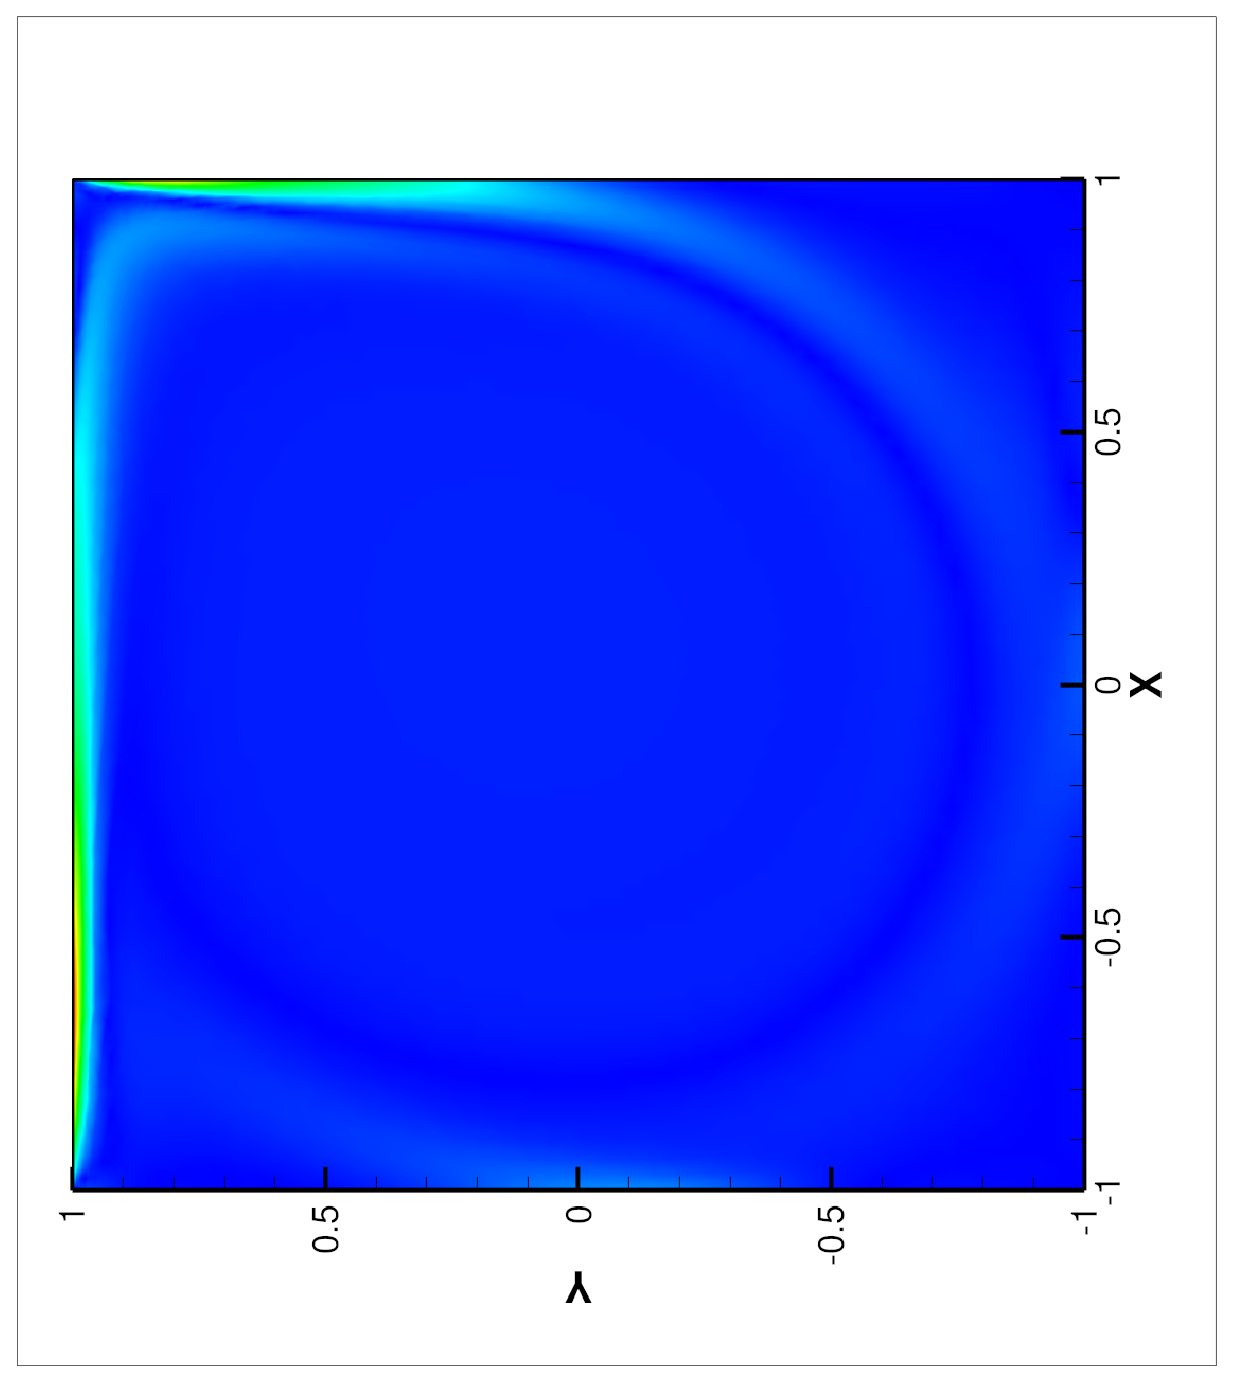
\includegraphics[width = 0.43\textwidth, angle = -90]{picture/cavity_flow_data/vortex.eps}
        \end{center}
        \caption{\small Cavity flow, left: mesh, right: vorticity
          contour, pressure mesh $40 \times 40$, $\nu = 0.001$.}
        \label{fig::cavity_flow_mesh}
       \end{figure}

       \begin{figure}[!htbp]
         \begin{center}
             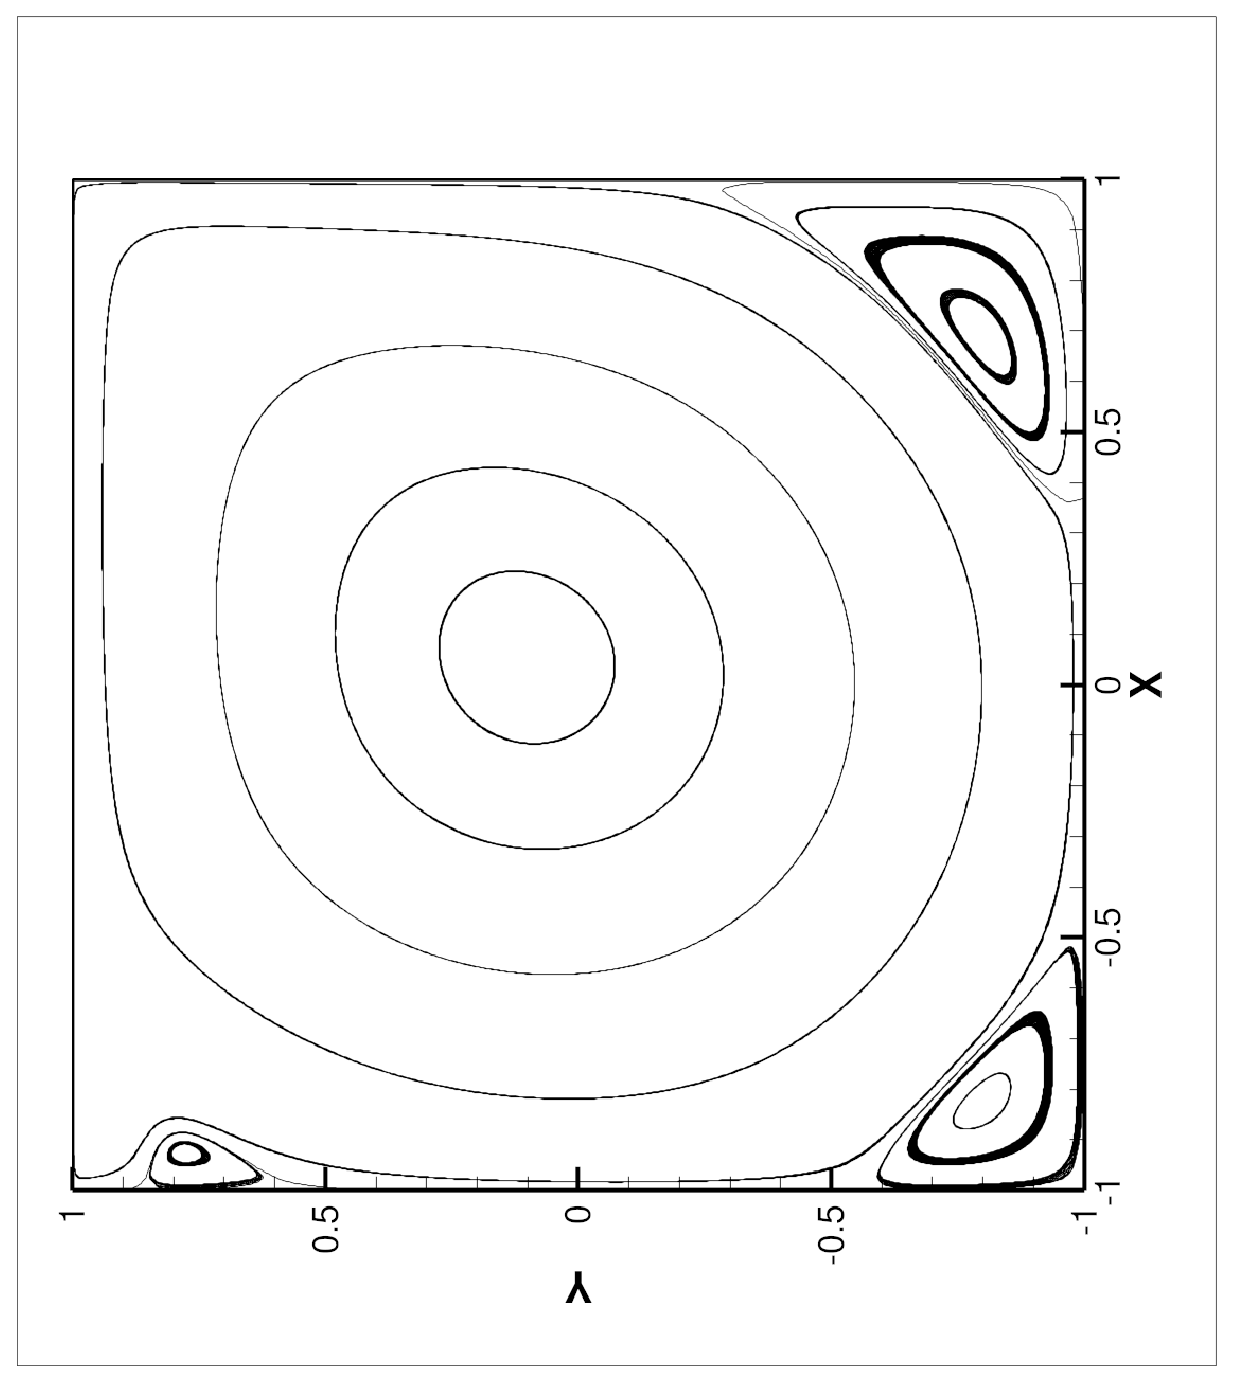
\includegraphics[width = 0.43\textwidth, angle = -90]{picture/cavity_flow_data/streamline.eps}
        \end{center}
        \caption{\small Cavity flow: velocity streamline, pressure
          mesh $40 \times 40$, $\nu = 0.001$.}
        \label{fig::cavity_flow_streamline}
       \end{figure}

       \begin{figure}[!htbp]
         \begin{center}
             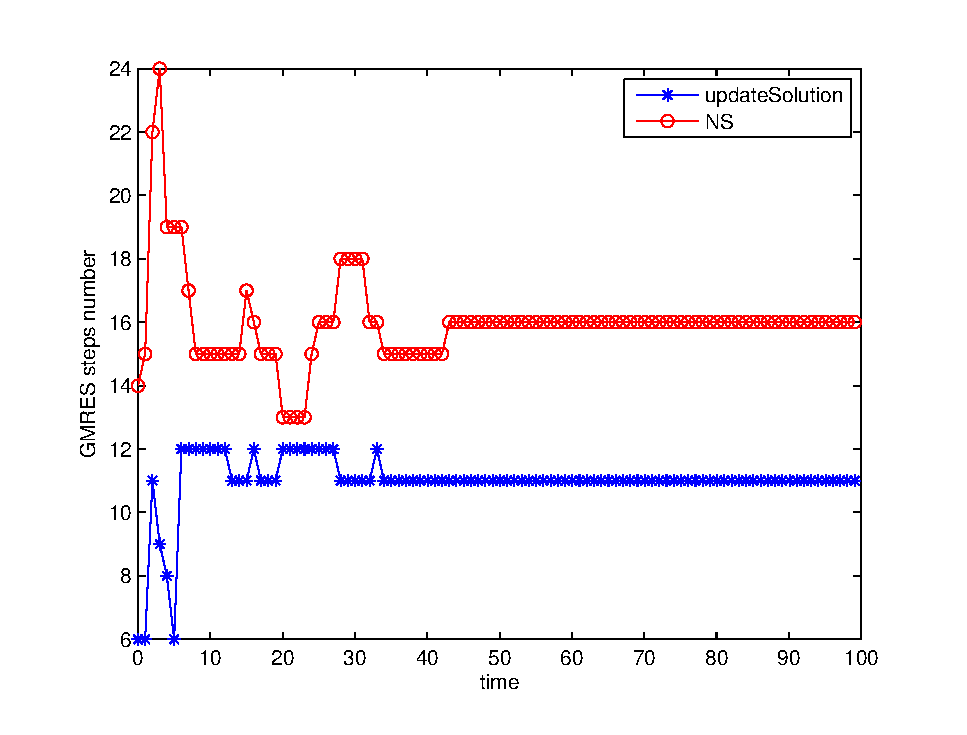
\includegraphics[width = 0.55\textwidth, angle = 0]{picture/cavity_flow_data/NS_iterate_steps.eps}
        \end{center}
        \caption{\small Cavity flow: GMRES step counts of solving
          (\ref{eq::linear_system}) with modified PCD preconditon.}
        \label{fig::cavity_GMRES_steps}
       \end{figure}
       
       \begin{table}[!htbp]
         \centering
         \begin{tabular}{cccc}
           \toprule
           \multirow{2}{*}{pressure mesh}    & \multirow{2}{*}{time
             step} & \multicolumn{2}{c}{GMRES step number} \\
           \cline{3-4}
            &               & $F_p = \nu A_p + W_p^n$ & $F_p = A_p + W_p^n$ \\ \midrule
           $20 \times 20$   &   $0.00656$         &      $41$           &     $8$
           \\ \midrule
           $40 \times 40$   &   $0.00312$         &      $43$           &     $12$
           \\ \midrule       
           $80 \times 80$   &   $0.00153$   &      $48$    &     $18$
           \\ \bottomrule 
         \end{tabular}
         \caption{Cavity flow: GMRES step number of solving linear system
           (\ref{eq::linear_system}) with different $F_p$ in PCD
           preconditioning at first time step, $\nu = 0.001$.}
         \label{tab::GMRES_steps_initial}
       \end{table}
   \subsection{Backward step flow}

      This example models the envolution of flow over a backward step.
      The length of the channel is $l = 5$. Poiseuille flow boundary
      condition $\vec{u} = (1 - y^2, 0)^T$is imposed on the inflow
      boundary $x = -1, y \in (0, -1)$. $\vec{u} = (0, 0)^T$ is imposed
      on the top and bottom walls while a natrual condition on the
      outflow boundary $x = 1, y \in (-1, 1)$. We choose viscosity
      $\nu = 0.02$, then the flow tends to steady as $t \rightarrow
      \infty$.
      
      We choose (\ref{eq::monitor_vorticity}) as monitor function
      with parameters $\alpha = 2.0, \beta = 2.0$. Singularities arise
      at the concave corner where flow expanding, so there needs more
      grids. In Figure \ref{fig::step_flow_mesh_streamline}, mesh
      clusters near the concave corner consistent with our assumption. 
      
      Our computational time step length is near $0.008$ which
      satisfing the CFL condition. GMRES iteration counts of solving
      system (\ref{eq::linear_system}) and
      (\ref{eq::full_discreted_update}) via time are shown in
      Figure \ref{fig::GMRES_steps_total}. It requires less than 21
      iteration steps in solving (\ref{eq::linear_system}). 
 
      \begin{figure}[!htbp]
        \centering
        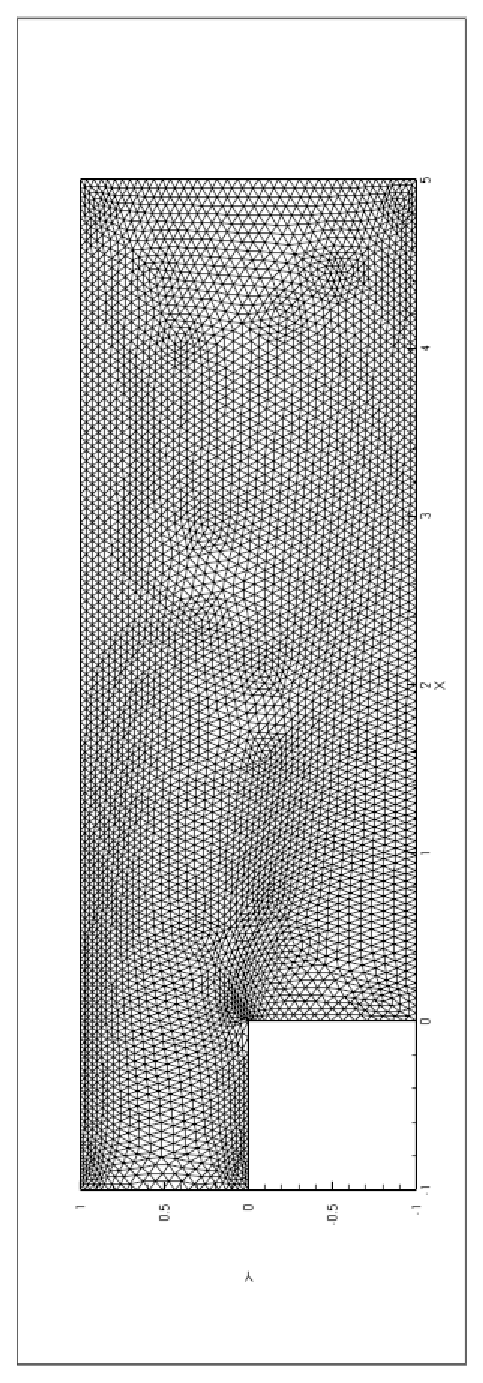
\includegraphics[width = 0.3\textwidth, angle =
        -90]{picture/L_shaped_flow_data/mesh.eps}
        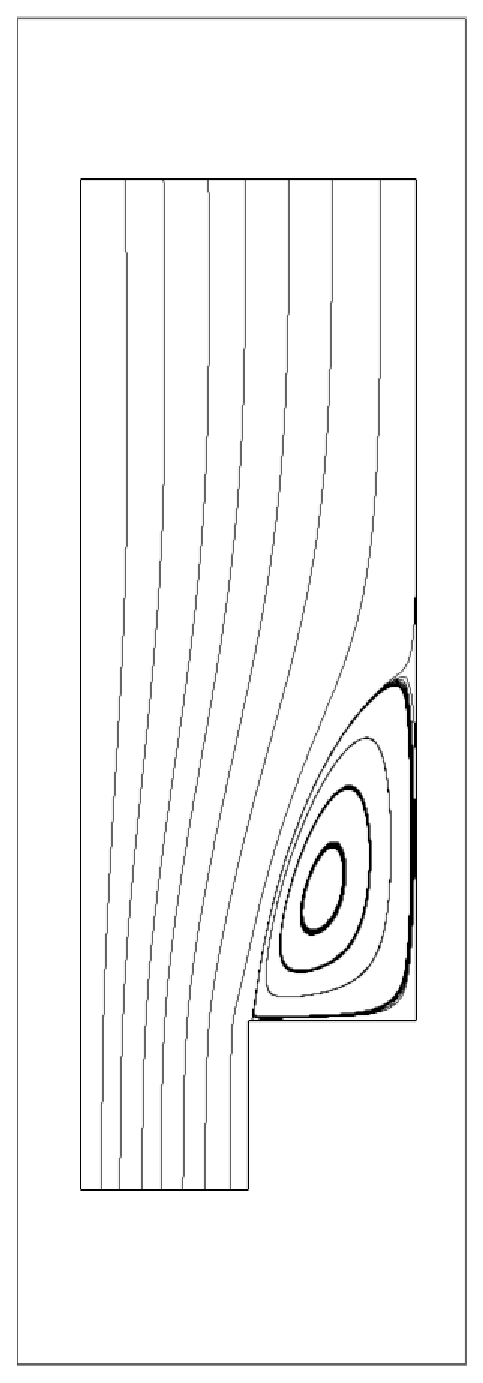
\includegraphics[width = 0.3\textwidth, angle =
        -90]{picture/L_shaped_flow_data/streamline.eps}
        \caption{\small Top: moving mesh, bottom: velocity streamline
          in step flow at $t = 100s$, viscosity $\nu = 0.02$.}
        \label{fig::step_flow_mesh_streamline}
      \end{figure}

      \begin{figure}[!htbp]
        \centering
        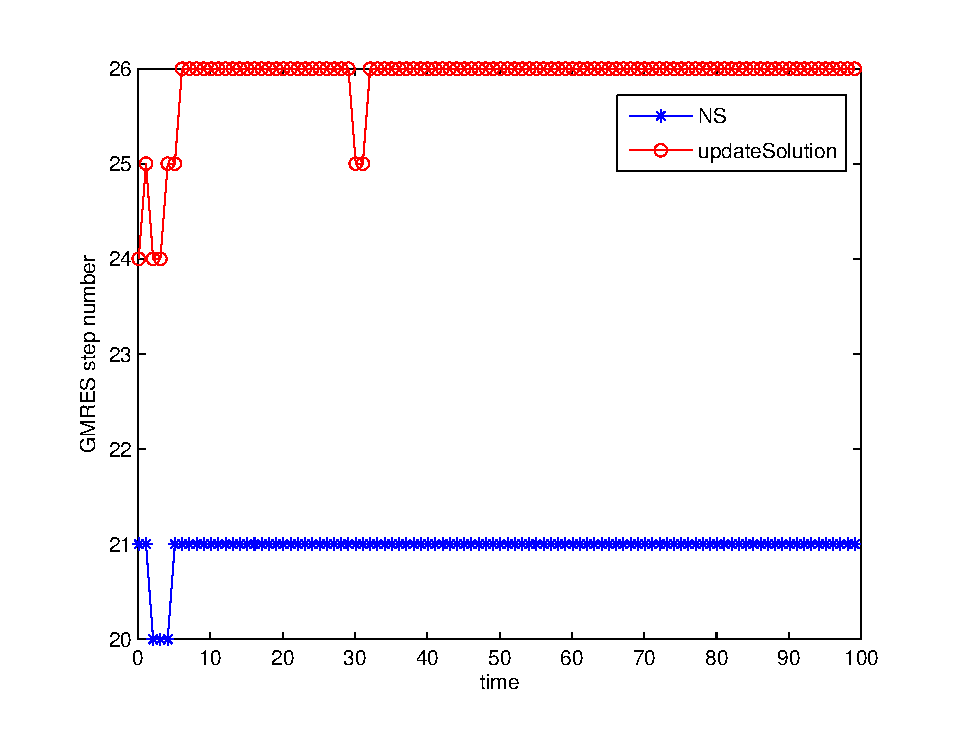
\includegraphics[width = 0.55\textwidth, angle = 0]{picture/L_shaped_flow_data/iterate_steps.eps}
        \caption{\small Step flow: GMRES iteration counts, $\nu = 0.02$}
        \label{fig::GMRES_steps_total}
      \end{figure}

   \subsection{Flow over cylinder}
   
      This example models the development of flow over an cylinder
      along a retangular channel. This problem has been considered in
      \cite{cao1999anr} with moving mesh method. The center of
      cylinder is $(0, 0)$ and the radius is $r = 0.3$. Let viscosity
      $\nu$  equal  $1 / 300$ and the domain $\Omega = [-1, 5] \times [-1, 1]$. 
      At the inflow boundary $x = -1$, $\vec{u} = (1 - y^2, 0)^T$ with
      poiseuille profile is imposed. On the top and bottom boundary
      of the channel, condition $\vec{u} = (0, 0)^T$ is
      settled. Natural condition is imposed on $x = 5$. 
      
      In our moving strategy, parameters $\alpha$ and
      $\beta$ in (\ref{eq::monitor_vorticity}) are user defined. The
      value of $\alpha$ is greater, the degree of mesh clustering is
      larger. From Figure \ref{fig::cylinder_GMRES_steps}, it can be
      shown that the number of GMRES iteration step with $\alpha = 5$
      is larger than $\alpha = 1.0$. Comparation of GMRES step counts between different
      choice of $F_p$ are shown in Figure 
      \ref{fig::cylinder_GMRES_steps_comparation}, it is found that
      the number of GMRES iteration steps will decrease more than 20 by  
      using $F_p = A + W_p^n$.

      We show the moving mesh at $t = 2s$ in Figure
      \ref{fig::cylinder_mesh_2s}. It can be seen that the mesh obviously
      clusters around the cylinder. As we known, wall street phenomena
      will occur as time evoluting when the flow has an appropriate
      viscosity, just as the mesh shown in Figure \ref{fig::cylinder_mesh_40s}.
      
      \begin{figure}[!htbp]
        \begin{center}
          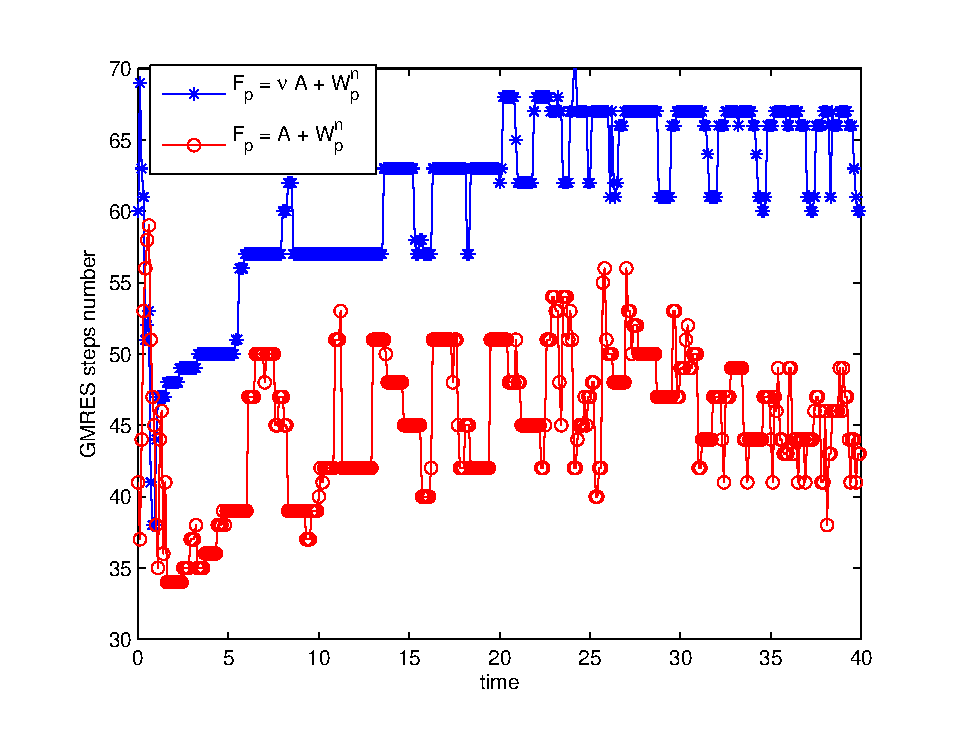
\includegraphics[width = 0.55\textwidth]{picture/obstacle_flow_data/comparation_NS_iterate_step.eps}
        \end{center}
        \caption{\small Flow over cylinder: GMRES iteration counts of
                 solving(\ref{eq::linear_system}) with different $F_p$ in
                 preconditioning, $\alpha = 5.0, \nu = 1/300$.}
        \label{fig::cylinder_GMRES_steps_comparation}
      \end{figure}
      
      \begin{figure}[!htbp]
        \begin{center}
          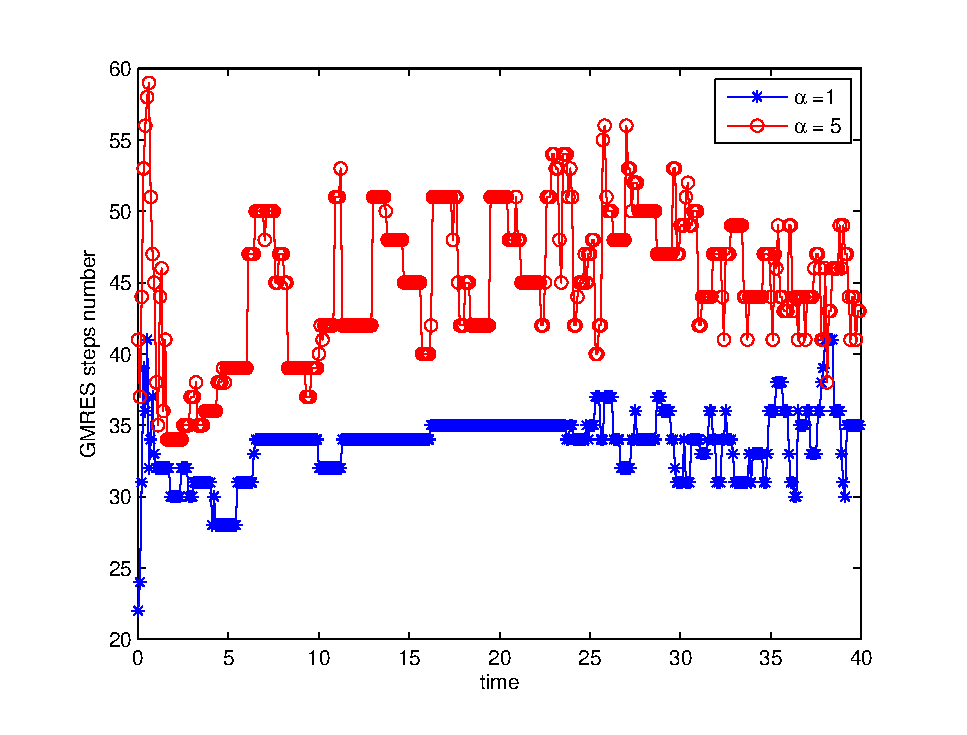
\includegraphics[width = 0.45\textwidth]{picture/obstacle_flow_data/NS_iterate_steps.eps}
          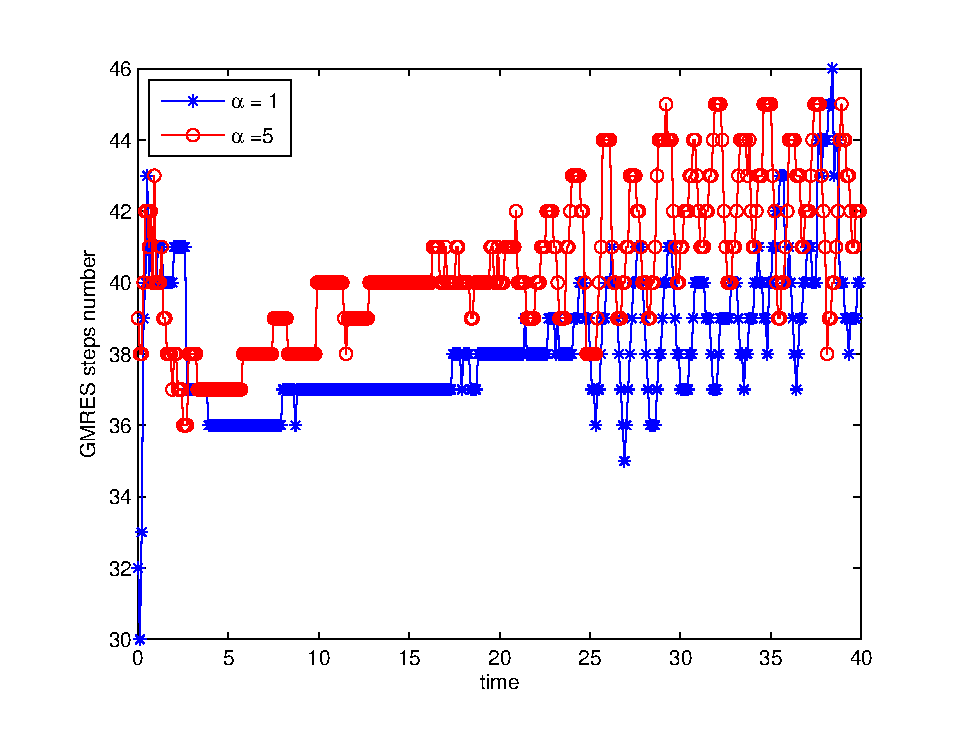
\includegraphics[width = 0.45\textwidth]{picture/obstacle_flow_data/moving_iterate_steps.eps}
        \end{center}
        \caption{\small Flow over cylinder, left: GMRES iteration counts of
          solving (\ref{eq::linear_system}), right: GMRES iteration
          counts of solving (\ref{eq::full_discreted_update}), $\nu =
          1/300$.}
        \label{fig::cylinder_GMRES_steps}
      \end{figure}
      
      
      \begin{figure}[!htbp]
        \centering
        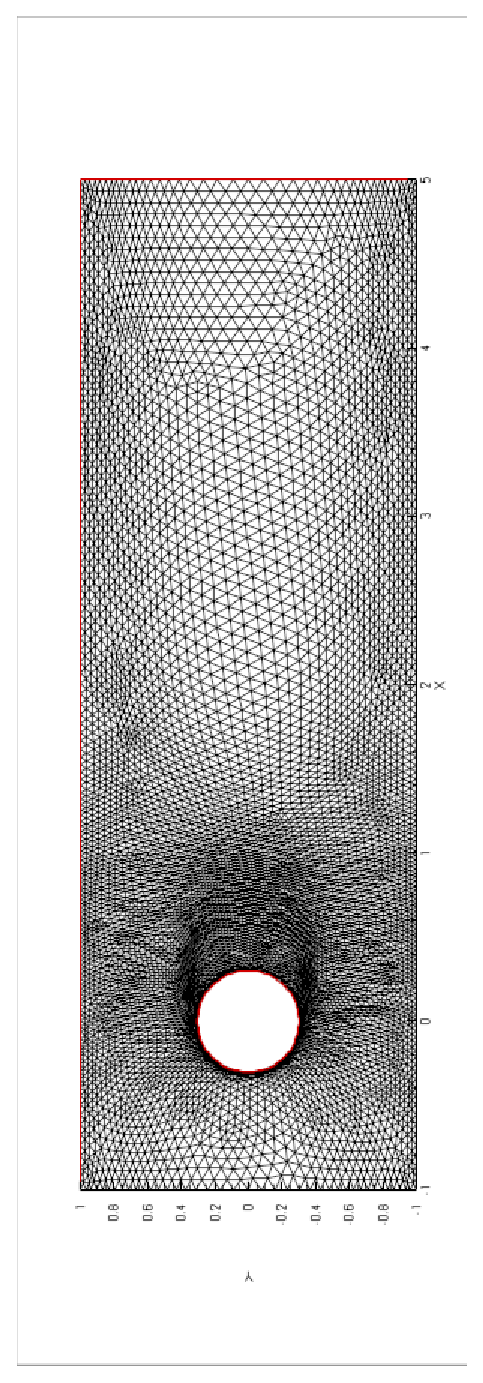
\includegraphics[width = 0.3\textwidth, angle = -90]{picture/obstacle_flow_data/mesh_t_2s.eps}
        \caption{\small Flow over cylinder: moving mesh at $t = 2s$,
          viscosity $\nu = 1/300$}
        \label{fig::cylinder_mesh_2s}
      \end{figure}

      \begin{figure}[!htbp]
        \centering
        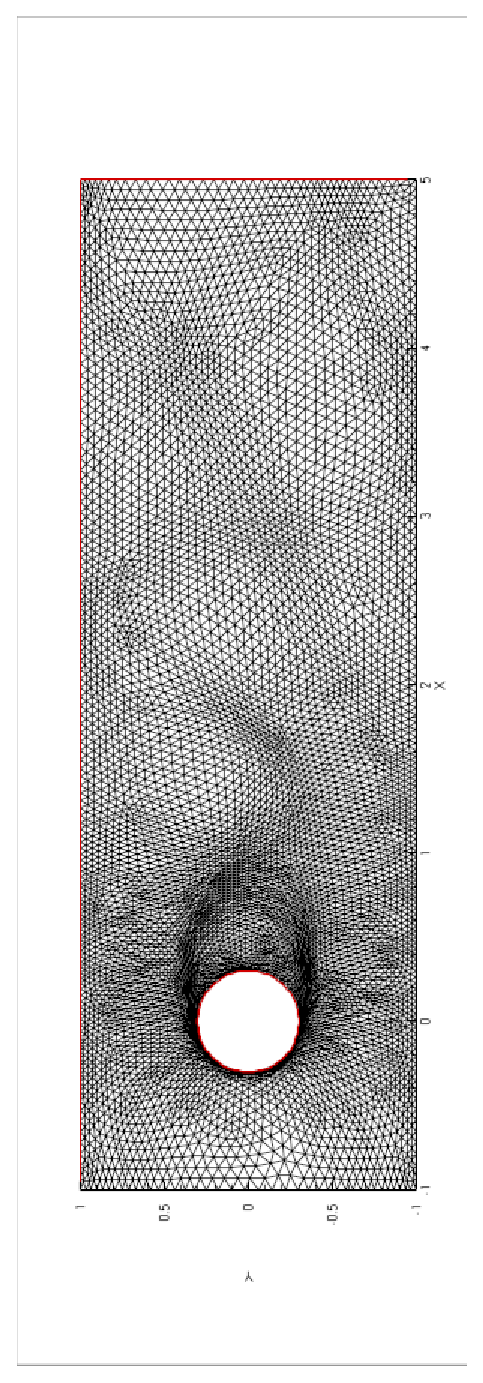
\includegraphics[width = 0.3\textwidth, angle = -90]{picture/obstacle_flow_data/mesh_t_40s.eps}
        \caption{\small Flow over cylinder: moving mesh at $t = 40s$,
          viscosity $\nu = 1/300$.}
        \label{fig::cylinder_mesh_40s}
      \end{figure}


%%% Remarks %%%%%%%%
\section{Remarks}
   \label{sec6} In this work, we apply an efficient AMG
   preconditioning strategy to moving mesh finite elment method based
   on $4P1-P1$ pair. The $4P1-P1$ element pair naturally satisfies the
   inf-sup condition and is linear-order. 
   Linear element is more prefered than high order element in
   practical engeneering computation, according to its simplicity and
   complexities of problems. In our moving strategy, we use the
   monitor function based on vorticity to capture the fine flow
   structure. The structure of mesh is consistent with vorticity
   structure. We compare the number of GMRES iterations of choosing
   different $F_p$ in PCD preconditioning. It is verified that
   modified PCD preconditioning is more efficient by three numerical
   tests. It is discoverd that the number of GMRES iteration step will
   be larger as the mesh becomes clustering. 
   
   We will extend the efficient preconditioning to some intrested 
   problems such as free boundary problem. Also three dimention
   problems of solving incompressible flow with moving mesh finite
   element based on $4P1-P1$ pair will be considered in future work. 

%%%% Acknowledgments %%%%%%%%
\section*{Acknowledgments}
The authors' work was supported in part by the National Basic Research
Program of China(2011CB309704) and the National Natrual Science
Foundation of China(11271358 and 91230108).
   
%%%% Bibliography  %%%%%%%%%%
\bibliographystyle{unsrt}
%include mathpaper.bib文件.
\bibliography{mathpaper}
% ----------------------------------------------------------------------------------------


 \end{document}
